\subsection{Modelli basati su Agenti}

I modelli basati su agenti rappresentano una metodologia computazionale 
utilizzata per simulare le azioni e le interazioni di un insieme di agenti 
autonomi, che possono essere individui o gruppi di individui. 
Lo scopo principale di tali modelli è comprendere il comportamento di un 
sistema e le relazioni che influenzano i suoi risultati \cite{7822080}.

Nella modellazione basata su agenti, un sistema viene suddiviso in un 
insieme di entità decisionali autonome chiamate "agenti". Ciascun agente 
valuta autonomamente la propria situazione e prende decisioni basate su 
un insieme di regole specifiche. Gli agenti possono eseguire una serie 
di comportamenti che sono appropriati per il sistema che rappresentano. 
Le interazioni competitive e ripetute tra gli agenti costituiscono una 
caratteristica distintiva di un modello basato su agenti, sfruttando la 
potenza computazionale dei computer per esplorare dinamiche altrimenti 
difficilmente accessibili attraverso la modellazione matematica tradizionale.

In una forma di base, un modello basato su agenti consiste in un sistema 
di agenti e delle relazioni tra di essi. Anche un modello estremamente 
semplice può rivelare comportamenti complessi e offrire informazioni 
preziose sulle dinamiche del mondo reale che stanno modellando.

Generalmente, gli agenti possono evolvere nel tempo, consentendo di 
osservare comportamenti precedentemente inaccessibili, noti come 
"comportamenti emergenti". I modelli più sofisticati spesso incorporano 
reti neurali, algoritmi evolutivi o altre tecniche di apprendimento per 
rendere la simulazione il più realistica possibile, tentando di 
incentivare la comparsa di queste tipologie di comportamenti.

L'uso di modelli basati su agenti in epidemiologia è noto da diversi 
decenni ed è stato utilizzato per simulare e comprendere una vasta gamma 
di problemi, spesso centrati sul comportamento umano come parametro chiave 
\cite{Bissett2021} \cite{El-Sayed2012-ac} \cite{Groff2019} \cite{Tracy2018-lc}. 
Uno dei parametri più rilevanti che è stato preso in considerazione è 
stato il comportamento sociale degli individui. Questo insieme di 
parametri comprende diverse interazioni specifiche, che possono essere 
raggruppate in macrocategorie se necessario.

Con l'avvento della pandemia di COVID-19, molti ricercatori si sono 
concentrati sulla creazione di modelli basati su agenti, sia puri che 
ibridi con equazioni differenziali, al fine di sviluppare simulazioni 
affidabili del decorso di una pandemia, tenendo conto di variabili 
stocastiche e imprevedibili come il comportamento umano. Questo approccio 
ha lo scopo di ottenere intuizioni sul comportamento emergente del sistema.

\begin{figure}[H]
    \begin{center}
        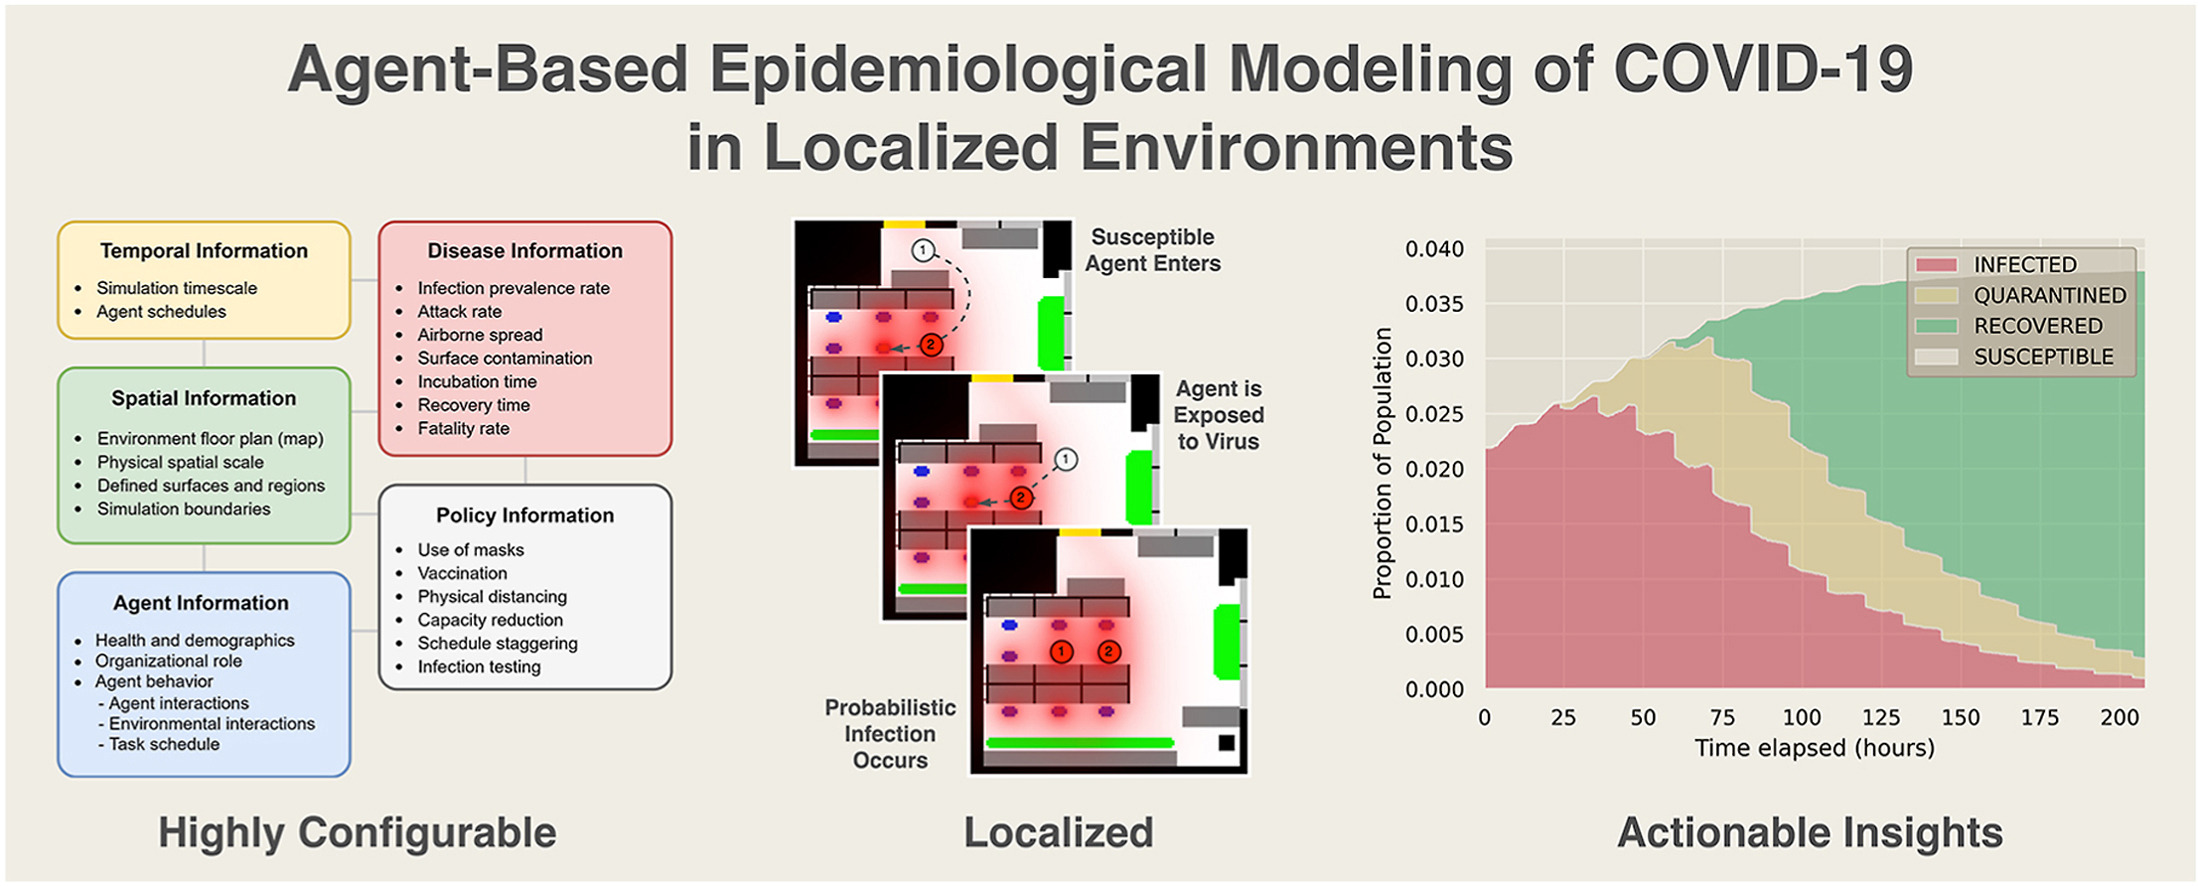
\includegraphics[width=\textwidth]{img/1-s2.0-S0010482522001883-ga1.jpg}
        \caption{Agent-Based Epidemiological Modeling of COVID-19 in Localized Environment \cite{CIUNKIEWICZ2022105396}}
        \label{fig:abm_covid}
    \end{center}
\end{figure}

\subsubsection{Comportamento Emergente}

I fenomeni emergenti sono il risultato delle interazioni tra singole entità. 
Non possono essere spiegati completamente attraverso le proprietà 
intrinseche delle singole parti, poiché dipendono dalle interazioni tra 
tali parti. Il comportamento emergente può manifestare proprietà separate 
dalle singole parti, rendendo la comprensione e la previsione del 
comportamento del sistema complesse, spesso contrarie all'intuito.

Un modello basato su agenti genera comportamenti emergenti dal basso verso 
l'alto, cioè dai singoli agenti all'intero gruppo. Ciò solleva domande 
sull'essenza stessa del comportamento emergente.

\begin{figure}[H]
    \begin{center}
        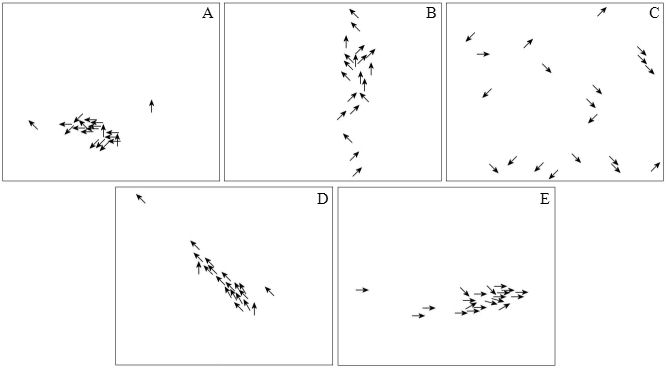
\includegraphics[scale=1]{img/Figure6b.jpg}
        \caption{Esempio di comportamento emergente nella simulazione degli stormi di uccelli}
        \url{https://www.jasss.org/13/2/8/Figure6b.jpg}
        \label{fig:flock_emergent_behaviour}
    \end{center}
\end{figure}

\subsubsection{Discretizzazione}

La discretizzazione è una delle sfide fondamentali nella simulazione, 
in quanto il mondo reale è continuo mentre gli strumenti di simulazione 
attuali operano su dati discreti. Durante la simulazione di eventi, 
è necessario decidere come adattare la realtà alla simulazione, 
con il rischio di perdere informazioni nel processo.

La discretizzazione in una simulazione può riguardare principalmente 
due aspetti: lo spazio e il tempo. Molti framework di simulazione offrono 
la possibilità di specificare come gestire la discretizzazione, 
ad esempio attraverso l'uso di parole chiave come "ContinuousSpace". 
Tuttavia, la scelta della discretizzazione può influenzare 
significativamente l'adeguatezza della simulazione per un dato contesto.

Va notato che la discretizzazione non è sempre negativa e che alcune 
simulazioni possono fornire risultati accurati anche con una 
discretizzazione significativa. La scelta della discretizzazione 
dipende spesso dalla specifica applicazione e dall'obiettivo della simulazione, nonché dai mezzi tecnici a disposizione.

\begin{figure}[H]
    \begin{center}
        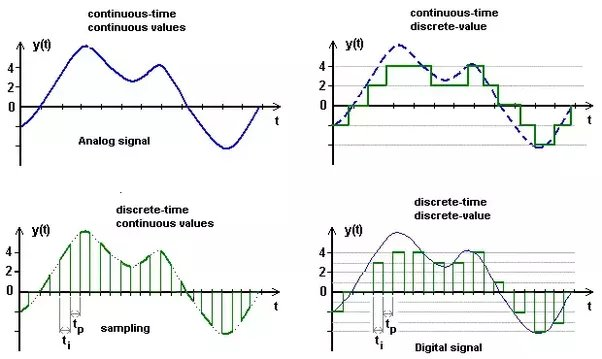
\includegraphics[scale=0.5]{img/main-qimg-100fc99cfe855462247225a07e1dfb7e-pjlq.jpg}
        \caption{Esempio di differenti tipologie di discretizzazione, siano esse nel tempo o nei valori}
        \url{https://qph.cf2.quoracdn.net/main-qimg-100fc99cfe855462247225a07e1dfb7e-pjlq}
        \label{fig:discretization}
    \end{center}
\end{figure}
